\documentclass{journal}[IEEEtran, twocolumn]             % No modificar

% PASO 1. Reemplace "Práctica 1" por el número de la práctica que corresponda
\newcommand{\dochead}{Práctica 1}     

% PASO 2. Reemplace "TÍTULO PRÁCTICA" por el título de la práctica que corresponda.
\newcommand{\docsubhead}{SDR y GNURADIO}  

% PASO 3. Reemplace "B1A - 02" por el grupo de la asignatura y el número de su grupo de laboratorio
\newcommand{\teamname}{C1}     

% PASO 4. OPCIONAL: Reemplace "\docsubhead \docsubhead" por el título del documento en caso de requerirse.
\newcommand{\titulo}{\dochead: \docsubhead}      

% PASO 5. Reemplace "31 de diciembre de 2030" por la fecha de su documento
\newcommand{\fecha}{8 de septiembre de 2024}      

% To load packages
\usepackage[T1]{fontenc}
\usepackage[utf8]{inputenc} 
\usepackage[spanish]{babel}
\usepackage[letter,left=2.0cm,top=2.0cm,right=2.0cm,bottom=4.0cm]{geometry}
\usepackage{amsmath}
\usepackage{amsfonts}
\usepackage{fancyhdr}
\usepackage{fancyvrb}
\usepackage{listings}
\usepackage{array}
\usepackage{graphicx,color,enumerate}	
\usepackage{multirow} 
\usepackage{multicol}
\usepackage{authblk}
\usepackage{charter}    % Font typeface
\usepackage{titling}
\usepackage{url}
\usepackage{hyperref}
\usepackage{xcolor}
\usepackage{booktabs}

\definecolor{uisgreen}{RGB}{125,194,3}
\definecolor{gray97}{gray}{.97}
\definecolor{gray75}{gray}{.75}
\definecolor{gray45}{gray}{.45}

\setlength{\droptitle}{-1.8cm}
\pagestyle{fancy}

%%% Header definition
\headheight=60pt 						% header height 
\renewcommand{\headrulewidth}{4pt}
\let\oldheadrule\headrule% Copy \headrule into \oldheadrule
\renewcommand{\headrule}{\color{uisgreen}\oldheadrule}

\fancyhead[L]							% left header 
{	\begin{minipage}{2.5cm}
		
\includegraphics[scale=0.3]{./figs/uislogohoriz.png} 
	\end{minipage}	
	\begin{minipage}{5cm}
	    \color{uisgreen}
	    \footnotesize {\textsf{Universidad Industrial de Santander\\ 
				Escuela de Ingenierías Eléctrica, \\
				Electrónica y de Telecomunicaciones	}}	
	\end{minipage}
}
\fancyhead[R] { 							%la "C" indica al centro
	\begin{minipage}{8cm}
	    \color{uisgreen}
	    \begin{flushright}
    	    \small{\textsf{Laboratorio de COMUNICACIONES I (27139)}} \\
            \normalsize{\textsf{\dochead: \textbf{\docsubhead}}} \\
    	    \small{\textsf{Grupo: \textbf{\teamname}}}
	    \end{flushright}
    \end{minipage}
    \begin{minipage}{1.2cm}
		
\includegraphics[width=1.0\textwidth]{./figs/logoE3T.png} 
	\end{minipage}	
}
%%% End header definition

\lstset{ frame=Ltb,
     framerule=0pt,
     aboveskip=0.5cm,
     framextopmargin=3pt,
     framexbottommargin=3pt,
     framexleftmargin=0.4cm,
     framesep=0pt,
     rulesep=.4pt,
     backgroundcolor=\color{gray97},
     rulesepcolor=\color{black},
     %
     stringstyle=\ttfamily\color{red!50!brown},
     showstringspaces = false,
     basicstyle=\small\ttfamily,
     commentstyle=\color{gray45},
     keywordstyle=\color{blue}\bfseries,
     %
     numbers=left,
     numbersep=15pt,
     numberstyle=\tiny,
     numberfirstline = false,
     breaklines=true,
   }

% minimizar fragmentado de listados
\lstnewenvironment{listing}[1][]
   {\lstset{#1}\pagebreak[0]}{\pagebreak[0]}

\lstdefinestyle{consola}
   {basicstyle=\scriptsize\bf\ttfamily,
    backgroundcolor=\color{gray75},
   }

\lstdefinestyle{C}
   {language=C,}             % No modificar


\begin{document}                    % No modificar

\title{\textbf{\titulo}}            % No modificar

% PASO 6. Agregar aquí el nombre y código de los autores.  
\author{
Sergio Camilo Santos Uribe - 2172315\\
Brayan Julian Niño Hurtado - 2172301\\
Carlos Alberto Cetina - 2215583\\
\href{https://github.com/scsantosdth/CommunicationsII_2024_2_scb.git}{https://github.com/scsantosdth/CommunicationsII_2024_2_scb.git}
}

\affil{\small{Escuela de Ingenierías Eléctrica, Electrónica y de Telecomunicaciones} \\ % No modificar
\small{Universidad Industrial de Santander}} % No modificar

\date{\fecha}                       % No modificar

\maketitle                          % No modificar
\thispagestyle{fancy}               % No modificar

%---------------------------------------------------------------
% PASO 7. **..**...****INICIE SU DOCUMENTO DESDE AQUI***...**...
%%%%% A PARTIR DE AQUÍ EDITE EL DOCUMENTO PARA AGREGAR TODO EL CONTENIDO REQUERIDO PARA EL ENTREGABLE CORRESPONDIENTE
%%%%  Todo el contenido a partir de este punto es SOLAMENTE ILUSTRATIVO.
%
% Para sus imformes, BORRE TODO el contenido de aquí en adelante  EXCEPTO la última línea que contiene el comando: \end{document}


\color{black}

\begin{multicols}{2}

\begin{abstract}
    En este laboratorio, se implementaron y analizaron bloques personalizados en GNU Radio para el procesamiento de señales, incluyendo un acumulador, un diferenciador y un bloque de promedios de tiempo. Estos bloques fueron evaluados con señales de entrada específicas, demostrando su correcta funcionalidad y su aplicabilidad en el análisis de señales en tiempo real. Los resultados obtenidos validaron la efectividad de estos bloques para tareas de acumulación, diferenciación y análisis estadístico de señales.

 \textit{\textbf{Palabras clave: GNU Radio, procesamiento de señales, acumulador, diferenciador, análisis estadístico.}} 
\end{abstract}

\section{Introducción}
   El objetivo es estudiar y entender la creación y evaluación de bloques personalizados en GNURADIO y en la aplicación de estos bloques en sistemas de tiempo real. En particular, el laboratorio incluye la implementación de bloques de acumulador y diferenciador, la creación de funciones para mostrar estadísticas específicas, y la propuesta y desarrollo de aplicaciones prácticas para señales reales. Este enfoque busca profundizar el conocimiento en SDR y mejorar las habilidades técnicas en programación de señales.


\section{Metodología}
\subsection{Parte A: Implementar los bloques acumulador y diferenciador}

Se programaron los algoritmos correspondientes para un bloque acumulador y un bloque diferenciador utilizando los bloques de Python en GNU Radio. Estos bloques fueron implementados generando un vector (1, 4, -2, -3) con el bloque vector source, como fuente de datos y los resultados se visualizaron mediante un bloque GUI Time Sink, que permitió observar en tiempo real la evolución de las señales procesadas por los bloques personalizados.

    \begin{center}
    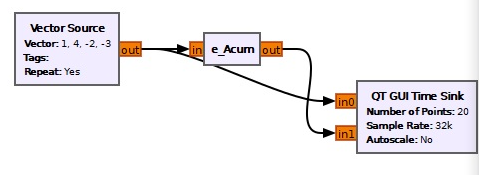
\includegraphics[width=0.45\textwidth]{figs/F1.png}
    \caption{Figura 1: Diagrama de flujo}
    \end{center}


\subsection{Parte B: Implementar bloque de estadísticas}

    Para evaluar el bloque de promedios de tiempo, se programó un bloque en GNU Radio que calcula varias métricas estadísticas de una señal de entrada. En este experimento, el bloque fue configurado para calcular la media, la media cuadrática, el valor RMS, la potencia promedio y la desviación estándar del vector de entrada (1,4,−2,−3). Los resultados se visualizaron utilizando un bloque Number Sink como se observa en la figura 2, que permite mostrar los valores calculados de cada métrica en tiempo real.
    
        \begin{center}
        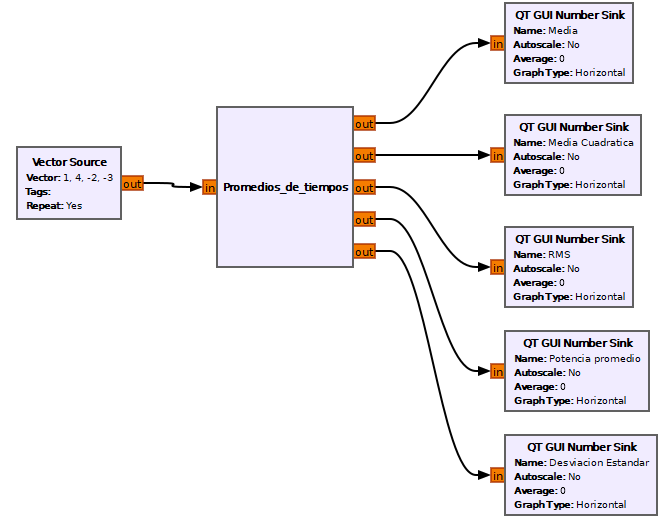
\includegraphics[width=0.45\textwidth]{figs/F4.png}
        \caption{Figura 2: Diagrama de flujo}
        \end{center}



\subsection{Parte C: Implementar aplicación y recrear vista de los resultados}
Se implementó una aplicación cuyo objetivo principal fue procesar una señal de audio. La aplicación consistió en ingresar una señal de audio y aplicar una serie de técnicas de filtrado y mejora para optimizar la calidad de la salida. Para lograr esto, se utilizaron los bloques previamente trabajados. Estos bloques permitieron realizar el análisis y procesamiento necesarios, pudiendo observar los promedios y gráficos de la señal de audio y sus características.

        \begin{center}
        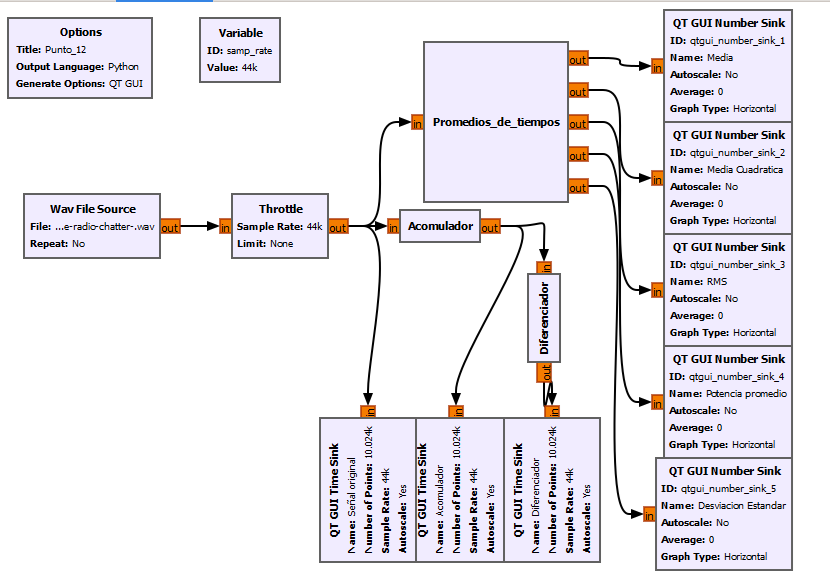
\includegraphics[width=0.45\textwidth]{figs/F6.png}
        \caption{Figura 3: Diagrama de flujo}
        \end{center}
    
\section{Resultados}
\subsection{Parte A: Implementar los bloques acumulador y diferenciador}
Como resultado del experimento, se generó una gráfica (Figura 4) que muestra dos señales distintas. La Señal 1 corresponde a la señal original con valores (1,4,−2,−3), mientras que la Señal 2 representa la salida del bloque acumulador, produciendo el vector (1,5,3,0). Este resultado confirma el correcto funcionamiento del bloque acumulador, el cual suma progresivamente los valores de la señal de entrada.

    \begin{center}
    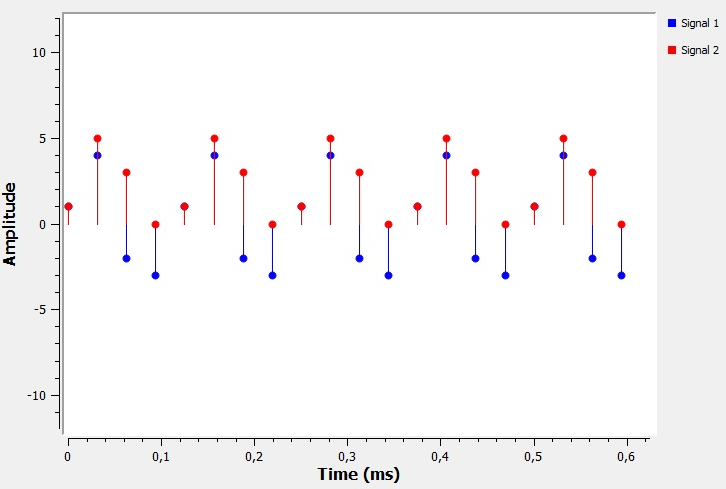
\includegraphics[width=0.45\textwidth]{figs/F2.png}
    \caption{Figura 4: Resultado bloque acumulador}
    \end{center}
    
    Para el caso del bloque diferenciador se obtuvo una salida con los valores (4,3,−6,−1). Esta salida refleja la correcta implementación del bloque diferenciador, el cual calcula la diferencia entre valores sucesivos de la señal de entrada. Específicamente, produciendo una salida que representa la tasa de cambio o la derivada discreta de la señal original (Figura 5).

    \begin{center}
    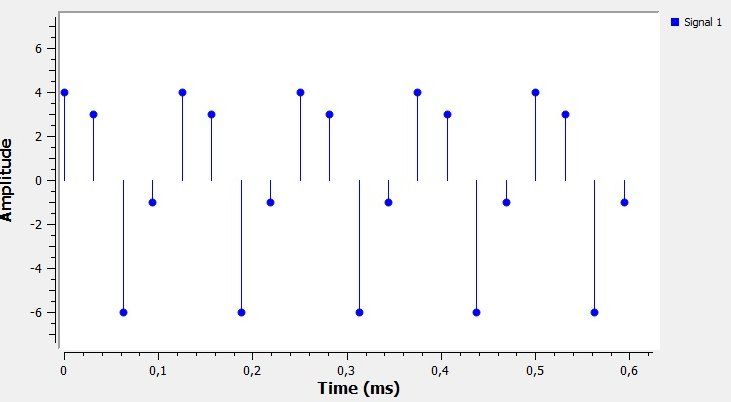
\includegraphics[width=0.45\textwidth]{figs/F3.png}
    \caption{Figura 5: Resultado bloque diferenciador}
    \end{center}
    
\subsection{Parte B: Implementar bloque de estadísticas}

    La aplicación del bloque de promedios de tiempo sobre el vector de entrada (1,4,−2,−3) proporcionó los siguientes resultados:
    \begin{itemize}
        \item Media: 0, que representa el promedio aritmético de los valores de la señal.
        \item Media Cuadrática: 7.5,calculada como la raíz cuadrada del promedio de los cuadrados de los valores.
       \item Valor RMS: \(\sqrt{7.5} = 2.7 \), que es la raíz cuadrada del promedio de los cuadrados de la señal.
        \item Potencia Promedio: 7.5 , obtenida como el promedio de los cuadrados de los valores de la señal.
        \item Desviación Estándar: 2.7 que mide la dispersión de los valores respecto a la media.
         
        \end{itemize}
        
        \begin{center}
        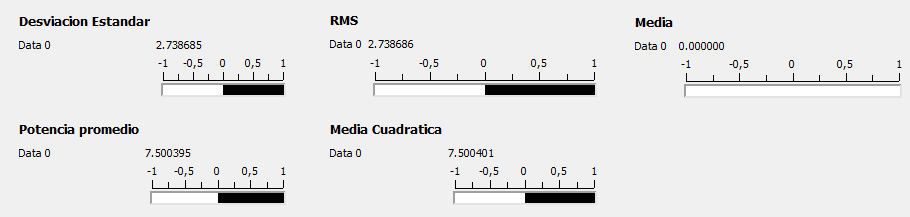
\includegraphics[width=0.45\textwidth]{figs/F5.png}
        \caption{Figura 6: Resultado bloque promedios de tiempo}
        \end{center}
        
\subsection{Parte C: Implementar aplicación y recrear vista de los resultados}
Como resultado, podemos observar las características de la señal: la gráfica de la integral, la derivada, los valores promedios, la media, la mediana cuadrática, el valor RMS, la potencia promedio y la desviación estándar de la señal.

  \begin{center}
    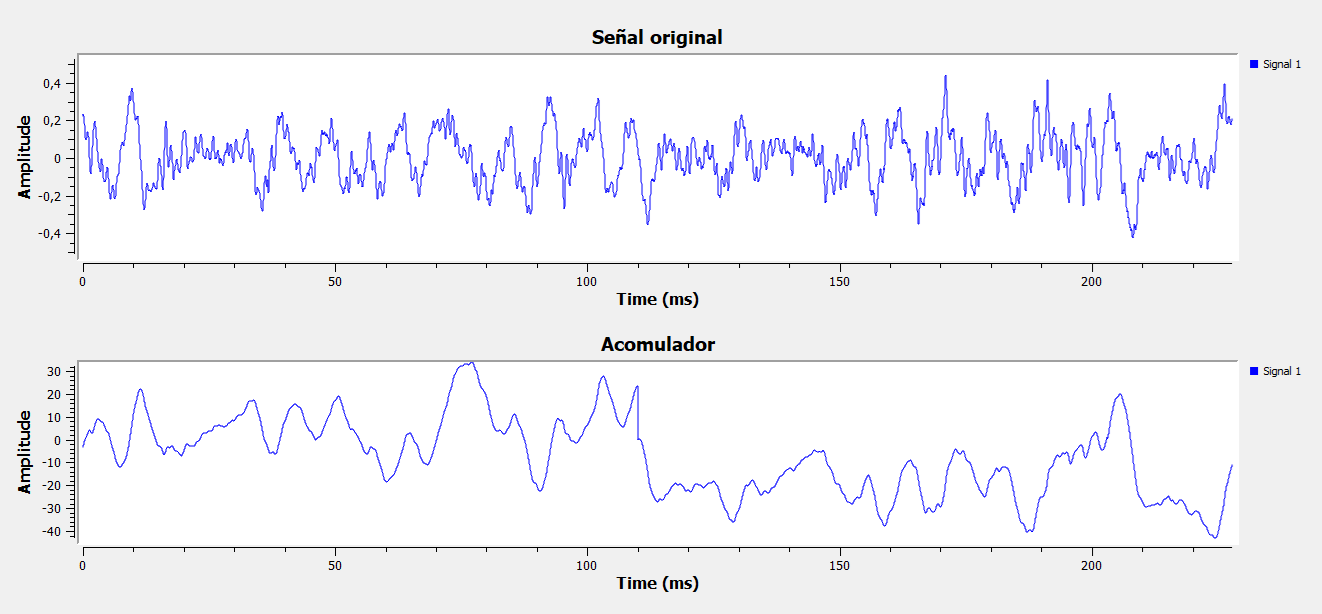
\includegraphics[width=0.45\textwidth]{figs/F7.png}
    \caption{Figura 7: Grafica de la señal y su integral}
    \end{center}
    
      \begin{center}
    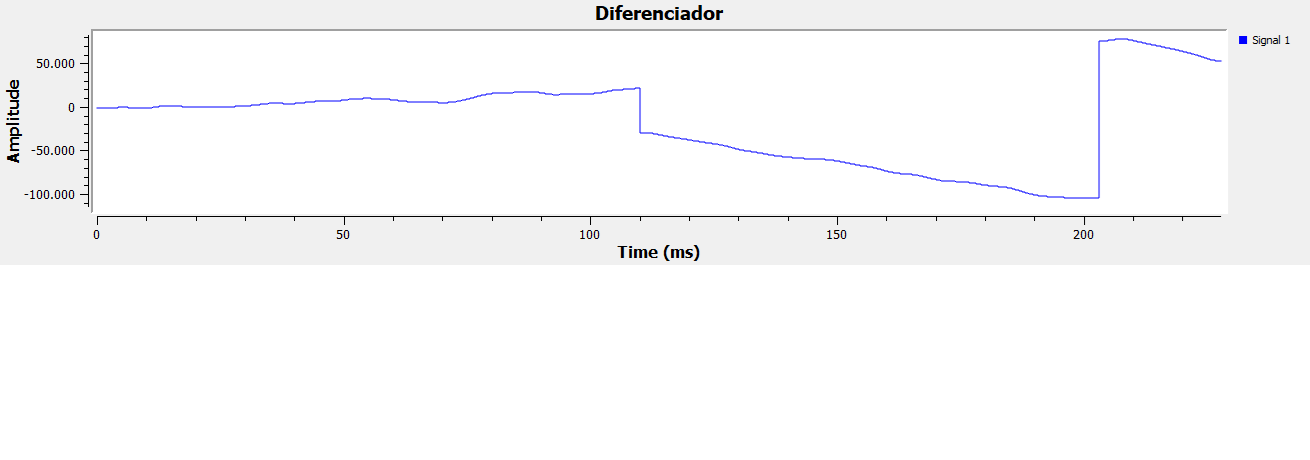
\includegraphics[width=0.45\textwidth]{figs/F8.png}
    \caption{Figura 8: Grafica de la derivada}
    \end{center}
    
      \begin{center}
    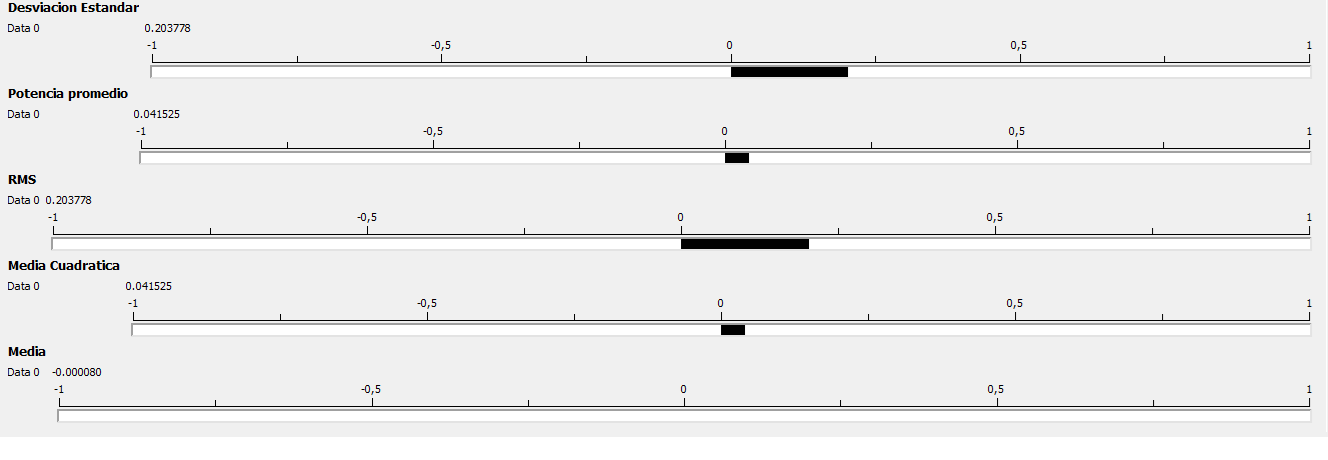
\includegraphics[width=0.45\textwidth]{figs/F9.png}
    \caption{Figura 9: Promedios de la señal}
    \end{center}


\section{Conclusiones}

\begin{itemize}
    
    \item La implementación y análisis del bloque acumulador demostraron su utilidad para generar una señal acumulativa, donde cada salida es la suma de los valores anteriores. Los resultados obtenidos evidencian la correcta operación del bloque, que es útil en aplicaciones como en la integración numérica o el análisis de tendencias en datos.
    
    \item El bloque diferenciador, por su parte, mostró su capacidad para calcular la diferencia entre valores consecutivos de una señal, proporcionando una nueva señal que representa la tasa de cambio o la derivada discreta de la señal original.
    
    \item La implementación del bloque de promedios de tiempo permitió calcular métricas estadísticas fundamentales como la media, la media cuadrática (RMS), la potencia promedio y la desviación estándar de una señal. Los resultados obtenidos validaron la precisión del bloque para ofrecer una visión cuantitativa de las propiedades estadísticas de la señal, lo cual es crucial en aplicaciones de procesamiento de señales donde es necesario caracterizar y comparar señales de manera objetiva.
    
\end{itemize}

\begin{thebibliography}{1}

\bibitem{comu} 
Homero Ortega and Óscar Reyes, "Comunicaciones Digitales basadas en radio definida por software", \textit{Editorial UIS}

\bibitem{wiki} 
Creating Your First Block:  \textit{https://wiki.
gnuradio.org/index.php?title=Creating_Your_First_Block}

\end{thebibliography}

\end{multicols}

\end{document}
